% Originally: content/week-02.tex, \subsection{Sequences and convergence} (Corsin Week 2, Monday)

\section{Sequences and convergence}
\label{sec:sequences_and_convergence}

% Transition: Claude Opus 5 (High)
Open and closed sets describe a space statically: which points sit comfortably inside a set and
which sit on its edge. Sequences describe the same thing dynamically, by asking where a moving
point ends up. The two descriptions turn out to be equivalent
(\cref{prop:open_closed_via_sequences}), and having both is what makes metric spaces pleasant to
work in. One description is usually easier to verify, the other easier to apply. Note that the
definition below is word for word the one from \emph{Analysis I}, with $|x_n - x|$ replaced by
$d(x_n,x)$. That substitution is the pattern for the whole chapter.

% Source: Corsin Nick/Class Notes/Week 2.pdf, pp. 1--13
\begin{definition}[Convergent sequence]
\label{def:convergent_sequence}
A \newterm{sequence} $(x_n)_{n=0}^{\infty}$ in a metric space $(X,d)$ is a function
$x : \mathbb{N} \to X$. We say that $(x_n)_{n=0}^{\infty}$ \newterm{converges} to $x \in X$ if
\[\forall \varepsilon > 0 \ \exists N \in \mathbb{N} \text{ such that } d(x_n, x) < \varepsilon \quad \forall n \geq N.\]
\end{definition}

\begin{center}
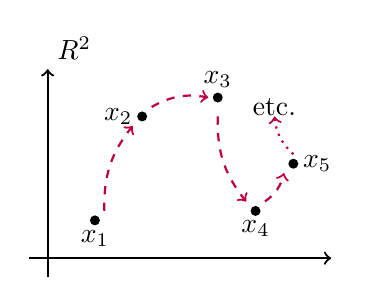
\begin{tikzpicture}[scale=1.2]
  % Axes
  \draw[->, thick] (-0.2, 0) -- (3, 0);
  \draw[->, thick] (0, -0.2) -- (0, 2);
  \node[anchor=south west] at (0, 2) {$\mathbb{R}^2$};

  % Sequence points
  \fill (0.5, 0.4) circle (1.5pt) node[below] {$x_1$};
  \fill (1.0, 1.5) circle (1.5pt) node[left] {$x_2$};
  \fill (1.8, 1.7) circle (1.5pt) node[above] {$x_3$};
  \fill (2.2, 0.5) circle (1.5pt) node[below] {$x_4$};
  \fill (2.6, 1.0) circle (1.5pt) node[right] {$x_5$};
  \node at (2.4, 1.6) {etc.};
  
  % Path
  \draw[->, purple, dashed, thick] (0.6, 0.5) to[bend left=20] (0.9, 1.4);
  \draw[->, purple, dashed, thick] (1.1, 1.6) to[bend left=20] (1.7, 1.7);
  \draw[->, purple, dashed, thick] (1.8, 1.5) to[bend right=20] (2.1, 0.6);
  \draw[->, purple, dashed, thick] (2.3, 0.6) to[bend right=20] (2.5, 0.9);
  \draw[->, purple, dotted, thick] (2.6, 1.1) to[bend left=20] (2.4, 1.5);
\end{tikzpicture}
\end{center}

% Supplement: Analysis_II_Script_v1.pdf, p. 7
\begin{notation}[\qt{Eventually}]
\label{not:eventually}
Let $(x_n)_{n\geq0}$ be a sequence in a set $X$ and let $\mathcal{P}$ be a property that a point
of $X$ may or may not have. One says $x_n$ satisfies $\mathcal{P}$ \newterm{eventually}
(\germanterm{schlie\ss lich}) if there exists $N \in \mathbb{N}$ such that $\mathcal{P}(x_n)$
holds for all $n \geq N$, or equivalently if $\mathcal{P}(x_n)$ fails for at most finitely many
$n$. In this vocabulary, \cref{def:convergent_sequence} reads: $(x_n)_n$ converges to $x$ if, for
every $\varepsilon>0$, $x_n$ eventually lies in $B_\varepsilon(x)$. The same compression applies
throughout the rest of this chapter and the next three.
\end{notation}

% Supplement: Sascha Brack/Class Notes/Week_02_Notes_Monday_Updated.pdf, p. 7
\begin{example}[A convergent sequence in $\mathbb{R}^3$]
\label{ex:convergent_sequence_R3}
Define a sequence $(x_n)_{n=1}^{\infty}$ in $\mathbb{R}^3$ by $x_n := \left(\frac{1}{n}, \frac{2}{n}, 1\right)$ for all $n \in \mathbb{N}$. Does a limit exist? If yes, what is it?
Yes, the sequence converges. Its limit can be computed coordinate-wise:
\[
\lim_{n\to\infty} x_n = \left(\lim_{n\to\infty} \frac{1}{n}, \lim_{n\to\infty} \frac{2}{n}, \lim_{n\to\infty} 1\right) = (0,0,1).
\]
\end{example}

% Sonnet 5 (Medium)
\begin{proposition}[Uniqueness of limits]
\label{prop:uniqueness_of_limits}
Let $(X,d)$ be a metric space. If a sequence $(x_n)_{n=0}^{\infty}$ in $X$ converges to both
$x \in X$ and $x' \in X$, then $x = x'$.
\end{proposition}

\begin{proof}
\begin{center}
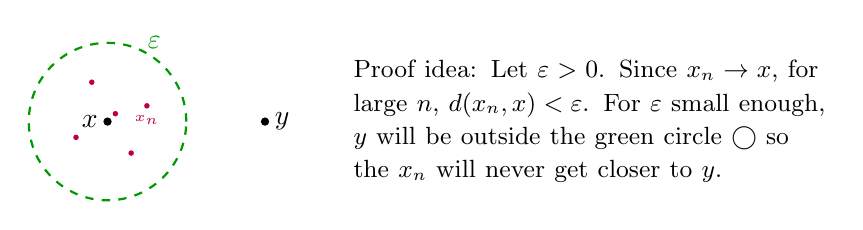
\begin{tikzpicture}
  \fill (0,0) circle (1.5pt) node[left] {$x$};
  \draw[green!60!black, dashed, thick] (0,0) circle (1);
  \node[green!60!black, above left] at (0.8, 0.8) {$\varepsilon$};
  
  \fill (2,0) circle (1.5pt) node[right] {$y$};
  
  \fill[purple] (0.5,0.2) circle (1pt) node[below] {\tiny $x_n$};
  \fill[purple] (0.3,-0.4) circle (1pt);
  \fill[purple] (-0.2,0.5) circle (1pt);
  \fill[purple] (-0.4,-0.2) circle (1pt);
  \fill[purple] (0.1,0.1) circle (1pt);
  
  \node[anchor=west, text width=6cm] at (3, 0) {
    \small Proof idea: Let $\varepsilon > 0$. Since $x_n \to x$, for large $n$, $d(x_n, x) < \varepsilon$. For $\varepsilon$ small enough, $y$ will be outside the green circle $\bigcirc$ so the $x_n$ will never get closer to $y$.
  };
\end{tikzpicture}
\end{center}
Fix $\varepsilon > 0$. By \cref{def:convergent_sequence}, there exist $N, N' \in \mathbb{N}$ such
that $d(x_n,x) < \varepsilon/2$ for all $n \geq N$ and $d(x_n,x') < \varepsilon/2$ for all
$n \geq N'$. For any $n \geq \max\{N,N'\}$, the triangle inequality (\cref{def:metric_space})
gives
\[d(x,x') \leq d(x,x_n) + d(x_n,x') < \varepsilon.\]
Since $\varepsilon > 0$ was arbitrary, $d(x,x') = 0$, so $x = x'$ by definiteness
(\cref{def:metric_space}).
\end{proof}

This justifies speaking of \qt{the} limit of a convergent sequence, as we do implicitly
throughout.

\begin{definition}[Accumulation point]
\label{def:accumulation_point}
Let $(x_n)_{n=0}^{\infty}$ be a sequence in a metric space $(X,d)$. A point $x \in X$ is an
\newterm{accumulation point} (\germanterm{H\"aufungspunkt}) of $(x_n)_{n=0}^{\infty}$ if some
subsequence $(x_{n_k})_{k=0}^{\infty}$ converges to $x$.
\end{definition}

% Supplement: Sascha Brack/Class Notes/Week_02_Notes_Monday_Updated.pdf, p. 3
\begin{remark}[A claim in the lecture script that is not fully correct]
The official lecture script states that a sequence converges to $x$ if and only if $x$ is its
\emph{only} accumulation point (\cref{def:accumulation_point}). Sascha Brack's class notes flag
this as false in general, with two counterexamples worth recording. First, a sequence can have a
unique accumulation point without converging: on $[0,1)$, let $x_{2n+1} := \tfrac1n$ and
$x_{2n} := 1-\tfrac1n$; the only accumulation point is $0$, yet $(x_n)$ does not converge, since
the terms $x_{2n} \to 1 \notin [0,1)$ leave every neighbourhood of $0$ infinitely often. Second,
even in $\mathbb{R}$ itself, the sequence with $x_n := \tfrac1n$ for odd $n$ and $x_n := n$ for
even $n$ has $0$ as its only accumulation point but is unbounded, hence divergent. What \emph{is}
true is the easier direction: if $(x_n)$ converges to $x$, then $x$ is its unique accumulation
point (this follows directly from \cref{prop:uniqueness_of_limits} together with the fact that
every subsequence of a convergent sequence converges to the same limit). The converse needs an
extra hypothesis, such as compactness of the ambient space (\cref{sec:compactness}) together with
some control ruling out the first counterexample's boundary-escaping behaviour.
\end{remark}

\begin{proposition}[Open/closed sets via sequences]
\label{prop:open_closed_via_sequences}
\begin{enumerate}[label=\textbf{(\alph*)}]
  \item $U \subseteq X$ is \textbf{open} if and only if, for every convergent sequence
    (\cref{def:convergent_sequence}) in $X$ with limit in $U$, the sequence eventually lies in
    $U$.
  \item $A \subseteq X$ is \textbf{closed} if and only if every convergent sequence in $A$ has its
    limit in $A$.
\end{enumerate}
\end{proposition}

% Generator: Claude Opus 5 (High) --- Corsin states this without proof, but it is the
% workhorse behind the uniform-convergence exercise below, so the argument is filled in here.
\begin{proof}
\begin{enumerate}[label=\textbf{(\alph*)}]
  \item \textbf{($\Rightarrow$)} Let $U$ be open and let $x_n \to x \in U$. Choose
    $\varepsilon>0$ with $B_\varepsilon(x) \subseteq U$ (\cref{def:open_closed}). By
    \cref{def:convergent_sequence} there is $N$ with $d(x_n,x)<\varepsilon$ for all $n \geq N$,
    so $x_n \in B_\varepsilon(x) \subseteq U$ from $N$ onwards.

    \textbf{($\Leftarrow$)} By contraposition. If $U$ is not open, some $x \in U$ has
    $B_{1/n}(x) \not\subseteq U$ for every $n \geq 1$, so we may pick
    $x_n \in B_{1/n}(x)\setminus U$. Then $d(x_n,x) < \tfrac1n \to 0$, so $x_n \to x \in U$, and
    yet \emph{no} term of the sequence lies in $U$.
  \item \textbf{($\Rightarrow$)} Let $A$ be closed, $(x_n)$ a sequence in $A$ with $x_n \to x$.
    If $x \notin A$, then $x$ lies in the open set $X\setminus A$, so by \textbf{(a)} the
    sequence eventually lies in $X\setminus A$, contradicting $x_n \in A$ for all $n$. Hence
    $x \in A$.

    \textbf{($\Leftarrow$)} We show $X\setminus A$ is open. If it were not, the same
    construction as in \textbf{(a)} yields $x \in X\setminus A$ and points
    $x_n \in B_{1/n}(x) \cap A$. Then $(x_n)$ is a sequence in $A$ converging to $x$, so the
    hypothesis forces $x \in A$, which is the required contradiction.
\end{enumerate}
\end{proof}

\begin{remark}[The shrinking-ball construction]
\label{rem:shrinking_ball_trick}
Both \qt{$\Leftarrow$} directions used the same device: negating \qt{some ball fits inside $U$}
gives a bad point in $B_{1/n}(x)$ for \emph{every} $n$, and collecting those points produces a
sequence converging to $x$. It is worth recognising, because it is the standard bridge from a
statement about balls to a statement about sequences, and it is exactly what makes
\cref{def:open_closed} and \cref{prop:open_closed_via_sequences} interchangeable in practice. In
the usual division of labour one proves closedness by the sequence criterion and openness by the
ball criterion.
Note that it needs the radii $\tfrac1n$ to shrink to $0$, which is where the metric enters;
in a general topological space the equivalence can fail.
\end{remark}

% Supplement: Analysis_II_Script_v1.pdf, p. 17
\begin{lemma}[Convergence is a topological notion]
\label{lem:convergence_is_topological}
Let $(X,d)$ be a metric space. A sequence $(x_n)_n$ in $X$ converges to $x$ if and only if, for
every open set $U \ni x$, $(x_n)_n$ eventually (\cref{not:eventually}) lies in $U$.
\end{lemma}

\begin{proof}
If $x_n \to x$ and $U \ni x$ is open, some $\varepsilon>0$ has $B_\varepsilon(x)\subseteq U$
(\cref{def:open_closed}), and $x_n$ eventually lies in $B_\varepsilon(x)$
(\cref{def:convergent_sequence}), hence in $U$. Conversely, taking $U := B_\varepsilon(x)$ itself
for each $\varepsilon>0$ recovers exactly \cref{def:convergent_sequence}.
\end{proof}

% Supplement: Analysis_II_Script_v1.pdf, p. 17
\begin{corollary}[Two metrics with the same topology have the same convergent sequences]
\label{cor:same_topology_same_convergence}
Let $X$ be a set endowed with two metrics $d_1$ and $d_2$. Then $(X,d_1)$ and $(X,d_2)$ have the
same convergent sequences if and only if the topologies they generate coincide.
\end{corollary}

\begin{proof}
By \cref{lem:convergence_is_topological}, whether $x_n \to x$ depends only on the collection of
open sets, that is, only on the topology $d_1$ or $d_2$ generates. Consequently, equal topologies
give equal convergent sequences.

For the converse, suppose $U \subseteq X$ is open with respect to $d_1$ but not with respect to
$d_2$; we exhibit a sequence distinguishing the two. Since $U$ is not $d_2$-open, some $x \in U$
has, for every $k \geq 0$, a point $x_k \in B^{d_2}_{2^{-k}}(x) \setminus U$. Then $x_k \to x$
with respect to $d_2$ (\cref{def:convergent_sequence}, since $2^{-k}\to0$), so by hypothesis also
$x_k \to x$ with respect to $d_1$. But $U$ is $d_1$-open and contains $x$, so
\cref{lem:convergence_is_topological} forces $(x_k)_k$ to eventually lie in $U$, contradicting
$x_k \notin U$ for every $k$. So every $d_1$-open set is $d_2$-open, and by symmetry the two
topologies coincide.
\end{proof}

\begin{remark}
This is the precise sense in which \qt{only the topology matters, not the metric itself} for
convergence. Two visibly different metrics, even one bounded and one unbounded, generate the same
convergent sequences exactly when they generate the same open sets, and one never has to compare
the metrics directly. \Cref{ex:2.5}\textbf{.2}'s three product metrics are one instance of this; so is
\cref{prop:concave_reshaping_metric} together with \cref{ex:reshaping_same_convergence}.
\end{remark}

% Source: Corsin Nick/Class Notes/Week 2.pdf, pp. 1--13
% (Re-cited: the proof and remark above this point are additions, not transcription.)
\begin{example}[Open, closed, and neither in $\mathbb{R}^2$]
\label{ex:open_closed_neither_R2}
In the euclidean metric space $\mathbb{R}^2$, and with
\cref{prop:open_closed_via_sequences} in hand, each answer is a one-line sequence argument:
\begin{enumerate}[label=\textbf{(\alph*)}]
  \item $[0,1]^2$ is \textbf{closed}: a sequence in $[0,1]^2$ converges coordinatewise
    (\cref{prop:Rn_coordinatewise_complete}), and each coordinate limit stays in $[0,1]$ because
    weak inequalities survive limits.
  \item $(0,1)^2$ is \textbf{open}: given $x \in (0,1)^2$, the distance from $x$ to the nearest
    edge is some $\varepsilon>0$, and $B_\varepsilon(x) \subseteq (0,1)^2$.
  \item $[0,1] \times (0,1)$ is \textbf{neither open nor closed}: it is not open because no ball
    around $(0,\tfrac12)$ fits inside it, and it is not closed because
    $(\tfrac12, \tfrac1n) \to (\tfrac12, 0)$ is a convergent sequence in the set whose limit is
    not.
\end{enumerate}
The picture below shows exactly these three witnesses. In \textbf{(a)} the escaping sequence stays
trapped, whereas in \textbf{(c)} one sequence escapes through the open edge while another does
not.
\end{example}

\begin{center}
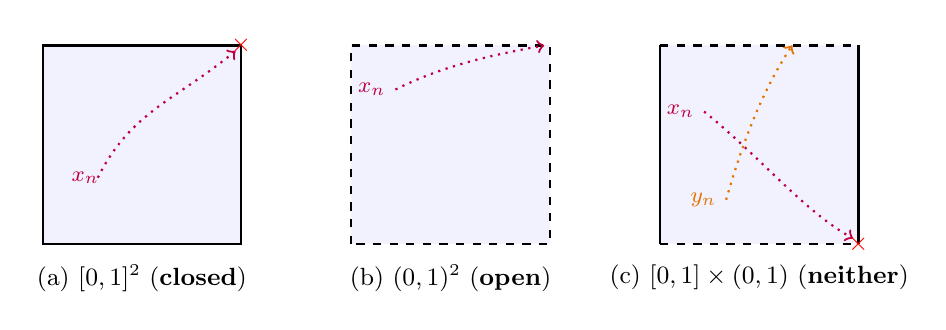
\begin{tikzpicture}[scale=1.4]
  % Panel 1: Closed
  \begin{scope}[shift={(0,0)}]
    \draw[thick, fill=blue!5] (0,0) rectangle (1.8,1.8);
    \draw[purple, thick, dotted, ->] (0.5,0.6).. controls (0.8,1.2) and (1.2,1.3).. (1.75,1.75);
    \node[purple, font=\footnotesize, left] at (0.6,0.6) {$x_n$};
    \node[red, font=\small] at (1.8,1.8) {$\times$};
    \node[below, font=\small] at (0.9,-0.1) {(a) $[0,1]^2$ (\textbf{closed})};
  \end{scope}

  % Panel 2: Open
  \begin{scope}[shift={(2.8,0)}]
    \draw[thick, dashed, fill=blue!5] (0,0) rectangle (1.8,1.8);
    \draw[purple, thick, dotted, ->] (0.4,1.4).. controls (0.8,1.6) and (1.2,1.7).. (1.75,1.8);
    \node[purple, font=\footnotesize, left] at (0.4,1.4) {$x_n$};
    \node[below, font=\small] at (0.9,-0.1) {(b) $(0,1)^2$ (\textbf{open})};
  \end{scope}

  % Panel 3: Neither
  \begin{scope}[shift={(5.6,0)}]
    \fill[blue!5] (0,0) rectangle (1.8,1.8);
    \draw[thick] (0,0) -- (0,1.8);
    \draw[thick] (1.8,0) -- (1.8,1.8);
    \draw[thick, dashed] (0,1.8) -- (1.8,1.8);
    \draw[thick, dashed] (0,0) -- (1.8,0);

    \draw[orange!90!black, thick, dotted, ->] (0.6,0.4).. controls (0.8,1.1) and (1.0,1.5).. (1.2,1.8);
    \node[orange!90!black, font=\footnotesize, left] at (0.6,0.4) {$y_n$};

    \draw[purple, thick, dotted, ->] (0.4,1.2).. controls (0.9,0.8) and (1.3,0.3).. (1.75,0.05);
    \node[purple, font=\footnotesize, left] at (0.4,1.2) {$x_n$};
    \node[red, font=\small] at (1.8,0) {$\times$};

    \node[below, font=\small] at (0.9,-0.1) {(c) $[0,1]\times(0,1)$ (\textbf{neither})};
  \end{scope}
\end{tikzpicture}
\end{center}

\begin{importantremark}[Common misconception!]
\label{rem:common_misconception}
In the euclidean metric space $X = [0,1]^2$, the set $[0,1]^2$ \textbf{is open}!
\begin{center}
\begin{tabular}{p{0.42\linewidth} p{0.42\linewidth}}
\textbf{$[0,1]^2 \subseteq \mathbb{R}^2$} & \textbf{$[0,1]^2 \subseteq [0,1]^2$} \\
Not open, since $B_\varepsilon(x)$ is not contained in $[0,1]^2$ if $x$ is on the boundary. &
Open, since the full space is always open, as shown before.
\end{tabular}
\end{center}
\end{importantremark}

\begin{center}
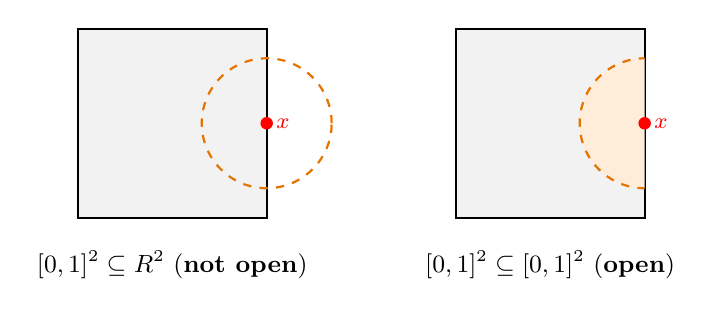
\begin{tikzpicture}[scale=1.5]
  % Panel 1: Ambient R^2
  \begin{scope}[shift={(0,0)}]
    \draw[thick, fill=gray!10] (0,0) rectangle (1.6,1.6);
    \fill[red] (1.6, 0.8) circle (1.5pt) node[right, font=\footnotesize] {$x$};
    \draw[orange!90!black, thick, dashed] (1.6,0.8) circle (0.55);
    \node[below, font=\small] at (0.8,-0.2) {$[0,1]^2 \subseteq \mathbb{R}^2$ (\textbf{not open})};
  \end{scope}

  % Panel 2: Ambient [0,1]^2
  \begin{scope}[shift={(3.2,0)}]
    \draw[thick, fill=gray!10] (0,0) rectangle (1.6,1.6);
    \begin{scope}
      \clip (0,0) rectangle (1.6,1.6);
      \draw[orange!90!black, thick, dashed, fill=orange!15] (1.6,0.8) circle (0.55);
    \end{scope}
    \fill[red] (1.6, 0.8) circle (1.5pt) node[right, font=\footnotesize] {$x$};
    \node[below, font=\small] at (0.8,-0.2) {$[0,1]^2 \subseteq [0,1]^2$ (\textbf{open})};
  \end{scope}
\end{tikzpicture}
\end{center}

\begin{exercise}[Uniform convergence]
\label{ex:uniform_convergence}
\begin{enumerate}[label=\textbf{(\alph*)}]
  \item Write down the definition of convergence of a sequence $(f_n)_{n=0}^{\infty}$ to $f$ in
    the metric space $X$ of bounded functions $[0,1] \to \mathbb{R}$ with the supremum metric.
  \item You know the resulting expression from Analysis 1. What is it called?
  \item \textit{(Optional)} Use the fact that $C^0([0,1]) \subseteq X$ is closed and
    \Cref{prop:open_closed_via_sequences} on \qt{sequentially closed} to conclude a big result
    from Analysis 1.
\end{enumerate}
\end{exercise}

% Kept inline: solved directly in Corsin Nick/Class Notes/Week 2.pdf, pp. 9--10.
\begin{exercisesolution}[Solution to \cref{ex:uniform_convergence}]
\begin{enumerate}[label=\textbf{(\alph*)}]
  \item $\displaystyle \forall \varepsilon > 0 \ \exists N \in \mathbb{N} : \sup_{x \in [0,1]} |f_n(x) - f(x)| < \varepsilon \quad \forall n \geq N$.
  \item This is \newterm{uniform convergence} (\germanterm{gleichm\"assige Konvergenz})!
  \item $C^0([0,1])$ is closed in the space of bounded functions with the supremum metric.

    \textit{Proof.} Let $f \in X \setminus C^0([0,1])$, i.e., $f : [0,1] \to \mathbb{R}$ is
    bounded and has at least one discontinuity at a point $x_0 \in [0,1]$. That is, we find
    $\varepsilon > 0$ such that for all $\delta > 0$ there exists $y \in (x_0 - \delta, x_0 +
    \delta)$ with $|f(x_0) - f(y)| \geq \varepsilon$. Then the $\tfrac{\varepsilon}{3}$-ball in
    $X$,
    \[
    B_{\varepsilon/3}(f) := \Big\{ g \in X : \sup_{x \in [0,1]} |f(x) - g(x)| < \tfrac{\varepsilon}{3} \Big\},
    \]
    is contained in $X \setminus C^0([0,1])$.

    \textit{Why:} let $g \in B_{\varepsilon/3}(f)$ and let $\delta > 0$ be arbitrary. Choose
    $y \in (x_0-\delta,\,x_0+\delta)$ with $|f(x_0)-f(y)| \geq \varepsilon$. Then
    \[\varepsilon \leq |f(x_0)-f(y)|
      \leq \underbrace{|f(x_0)-g(x_0)|}_{<\ \varepsilon/3}
         + |g(x_0)-g(y)|
         + \underbrace{|g(y)-f(y)|}_{<\ \varepsilon/3},\]
    so $|g(x_0)-g(y)| > \varepsilon/3$. As $\delta$ was arbitrary, $g$ is discontinuous at
    $x_0$ too, i.e.\ $g \notin C^0([0,1])$. The whole point of the $\tfrac{\varepsilon}{3}$ is
    that two of the three terms are spent on moving from $f$ to $g$ and back, leaving a third
    of the jump behind.

    Given this fact, \cref{prop:open_closed_via_sequences} ensures that the uniform limit $f$ of
    $(f_n)_{n=0}^{\infty}$ in $C^0([0,1])$ is also in $C^0([0,1])$, i.e., continuous, given that
    $f : [0,1] \to \mathbb{R}$ is bounded. This is the case, since $f_n$ is bounded for all
    $n \in \mathbb{N}$, and with $\varepsilon = 1$ we find $N \in \mathbb{N}$ such that
    \[
    \sup_{x \in [0,1]} |f_N(x) - f(x)| < 1,
    \]
    which implies that $f$ is bounded.
\end{enumerate}
\end{exercisesolution}

\begin{center}
\begin{tikzpicture}[>=Latex, scale=1.4]
  \draw[->] (-0.2,0) -- (3.2,0) node[right] {$x$};
  \draw[->] (0,-0.2) -- (0,2.2) node[above] {$y$};
  \draw (0,0.05) -- (0,-0.05) node[below, font=\footnotesize] {$0$};
  \draw (2.6,0.05) -- (2.6,-0.05) node[below, font=\footnotesize] {$1$};

  \draw[blue!80!black, thick] plot[domain=0:2.6, samples=50] (\x, {1.0 + 0.3*sin(\x r * 2.5)});
  \node[blue!80!black, right] at (2.6, 1.06) {$f(x)$};

  \draw[red!80!black, thick, dotted] plot[domain=0:2.6, samples=50] (\x, {1.0 + 0.35 + 0.3*sin(\x r * 2.5)});
  \draw[red!80!black, thick, dotted] plot[domain=0:2.6, samples=50] (\x, {1.0 - 0.35 + 0.3*sin(\x r * 2.5)});

  \draw[orange!90!black, <->, thick] (1.3, 0.5) -- node[right, font=\footnotesize] {$\frac{2\varepsilon}{3}$} (1.3, 1.2);
  \node[red!80!black, font=\small, above] at (1.3, 1.8) {$B_{\varepsilon/3}(f)$ ($\varepsilon$-tube)};
\end{tikzpicture}
\end{center}
